\chapter{Particle identification}
\label{ch:pid}

\code{AtPIDTask} (in \code{AtReconstruction/}) turns every pattern-recognized track into PID observables: a
rigidity \brho{} and a specific energy loss \sqdedx. The estimators live in \code{AtTools/AtPID/}. The task writes
one \code{AtPIDEvent} per event, holding one result per track and per estimator. The vectors are parallel, but
downstream code must match on \code{trackID}, never on the array position (the track IDs of
\code{AtTrackFinderTC} are cluster labels).

\section{The PID variable}

For a singly charged ion, \dedx{} is proportional to $1/\beta^2$ in the Bethe--Bloch regime, so
$\sqrt{\mathrm{d}E/\mathrm{d}x}\propto 1/\beta$, and with $B\rho = p = m\beta\gamma$,
\begin{equation}
  \ln\!\left(\sqrt{\mathrm{d}E/\mathrm{d}x}\;B\rho\right) = \ln(m\gamma) + \text{const}.
\end{equation}
This \emph{ln-mass} variable places protons, deuterons and tritons $\ln 2 = 0.69$ and $\ln 1.5 = 0.405$ apart. An
ion of charge $z$ has $B\rho = p/z$ and \dedx{} $\propto z^2$, so $^4$He lands at $\ln(m_\alpha/m_d) = 0.69$ above the
deuterons, and $^3$He coincides with tritons. Gates are drawn on the plane \sqdedx{} against \brho, or on the ln-mass
distribution in slices of \brho.

\section{Estimators}

\begin{center}
\small
\begin{tabular}{p{0.18\textwidth}p{0.34\textwidth}p{0.39\textwidth}}
\toprule
Estimator & Method & Strengths and failure modes \\
\midrule
\code{AtPIDEstimator} (\code{GetClassic()}) & total charge over arc length & inflated \dedx; kept only for comparison \\
\code{AtSpyralPID} (\code{GetSpyral()}, \code{GetDefault()}) & port of the Spyral method: hits sorted in $z$, a spline
  along the track, a circle fitted to the first arc; \dedx{} over the first arc on the small pads &
  sharpest \dedx{} on well-measured tracks. Fails on tracks nearly flat in $z$, whose radius can come out much too
  large (Sec.~\ref{sec:pid-combine}); \code{SetMinPoints} (default 30) rejects many tracks (knee at 15--20);
  \code{SetZTieTolerance} avoids a singular spline on $z$ ties \\
\code{AtHelix3D} (\code{GetHelix3D()}) & hits ordered in 3D along a minimum-spanning-tree backbone, helix fitted at
  each end, vertex end by a two-of-three vote (rotation sense, Spyral direction, Bragg rise); \dedx{} = charge over the
  helix path of the first arc on the small pads &
  independent of the $z$ ordering; robust direction; supplies range, containment and charge-profile flags. Its circle
  averages a radius that shrinks along a slowing track, so the \brho{} of stopping tracks is biased low, more for
  heavier species \\
\bottomrule
\end{tabular}
\end{center}

\code{AtPIDTask} runs all three. \code{SetRunHelix3D(false)} skips the 3D estimator. \code{SetBField} and
\code{SetSmallPadRadius} (default 152~mm) are passed to every estimator; \code{SetZPadPlane} sets the lab-frame
transform of the 3D estimator ($z_\mathrm{lab} = z_\mathrm{pad\,plane} - z_\mathrm{digi}$; the default is 1000~mm, see
Chapter~\ref{ch:conventions}).

\subsection{AtHelix3D options}

\begin{center}
\small
\begin{tabular}{p{0.3\textwidth}p{0.15\textwidth}p{0.47\textwidth}}
\toprule
Setter & Default & Purpose \\
\midrule
\code{SetHitRefit(circle, alsoZ)} & off & refit the vertex-end circle (and $z(\phi)$) on the raw window hits instead of
  the 4~mm centroids; better precision \\
\code{SetArcAngle(on, frac)} & off, 0.5 & polar angle from $z_\mathrm{lab}$ against the arc length round the
  vertex-end circle, over the first \code{frac} of the window hits; stores \code{thetaArc} and
  \code{brhoArc} $= BR/\sin\theta$. Unbiased on simulation to 0.2--0.3\,\% in $\sin\theta$. Use with
  \code{SetHitRefit(true, true)} \\
\code{SetContainment(rMax, zMin, zMax)} & 145, 10, 955~mm & \code{contained}: the far-end centroid is inside the gas.
  The $z$ limit matters: tracks leaving the end of the drift window otherwise look contained. Re-measure per set-up \\
\code{SetMidPeak(fpk, after, tail)} & 0.75, 30~mm, 0.35 & \code{midPeak}: the charge profile peaks before
  \code{fpk} of the track, more than \code{after} before its end, and the mean after the peak is below \code{tail}
  times the peak -- a stopped particle with other hits attached \\
\code{SetExpectedSense} & $+1$ & rotation sense used by the direction vote; measure it for each field, charge and
  geometry \\
\code{SetEndWindowCap}, \code{SetAxisConstraint}, \code{SetRadiusGuard}, \code{SetBlobRemoval}, \code{SetBraggVote} &
  see header & vertex-end window and robustness options \\
\bottomrule
\end{tabular}
\end{center}

The fields \code{length} (the range of a stopping track), \code{rStop}, \code{zLabStop}, \code{peakFrac},
\code{tailRatio}, \code{contained} and \code{midPeak} are filled for every track whose backbone could be built.
The centroids inside the estimator are in the transformed frame $z' = z_\mathrm{sign} z + z_\mathrm{offset}$; code
that compares them with raw hits must transform the hits.

\section{Calibration}
\label{sec:pid-calib}

\paragraph{Per-run gain.} The detector gain drifts over a campaign; on a1975 the deuteron band moved by 0.12 in
ln-mass between the first and the last run (gain $-20$\,\%). Without a correction every band is smeared and a fixed
gate is off-centre for some runs. The factors are produced from the data (for example the position of the elastic
deuteron band at fixed kinematics, \code{macro/Unpack\_HDF5/a1975/D2\_UKF/pid\_gain\_norm.C}), stored in a text table
read by \code{AtTools::AtPIDGainTable} (\code{run gainSpyral gain3D} per line), and applied with
\code{AtPIDTask::SetDedxGain(gSpyral, g3D)}. A run that is missing from the table returns $-1$, so that a production
fails loudly rather than running uncorrected.

\paragraph{Pad gain.} \code{AtPIDTask::SetPadGainMap(file, column)} divides every hit charge by its pad's relative gain
before any estimator runs (on a copy of the track; the pattern event is untouched). The map, one \code{pad value}
line per pad, is read by \code{AtPIDGainTable::LoadPadGains}. On a1975 it was measured from the hit amplitudes of
each track relative to the track median (\code{pad\_gain\_map\_dp.C}); it shows a gain depression near the beam axis
that is absent in the simulation (Fig.~\ref{fig:pid-padgain}) and narrows the bands by 4--7\,\%.

\begin{figure}[htbp]
  \centering
  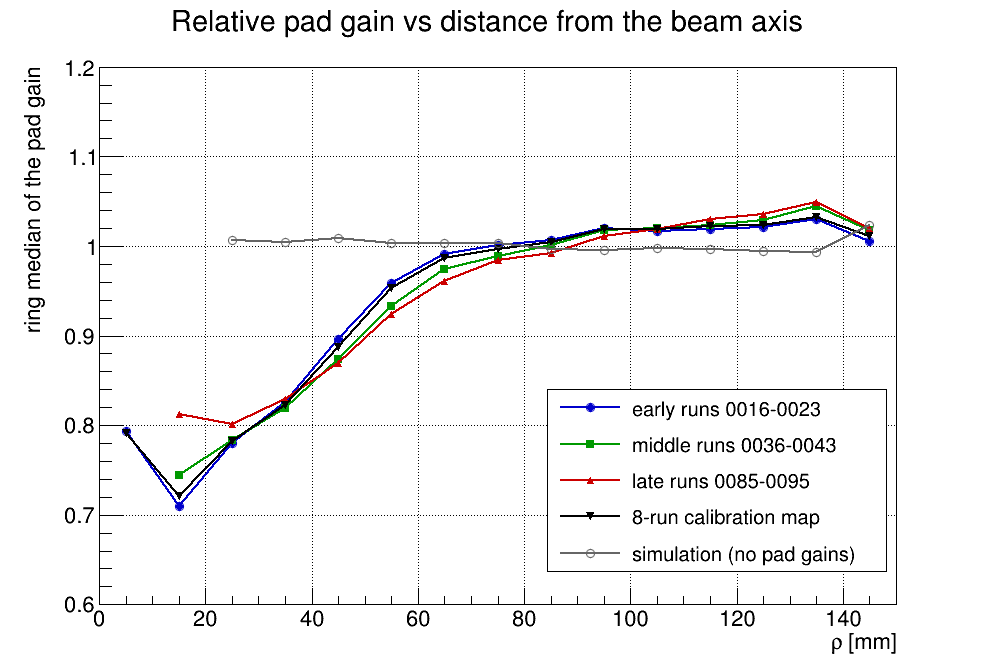
\includegraphics[width=0.65\textwidth]{figures/padgain_radial.png}
  \caption{Radial profile of the a1975 pad-gain map for three periods of the campaign.}
  \label{fig:pid-padgain}
\end{figure}

\paragraph{Saturation.} The GET electronics saturate. Slow, heavily ionising tracks lose charge in their PID segment
(a1975: about 21\,\% of the segment of deuterons at \brho{} 0.15--0.20~T\,m). The simulation does not saturate unless
\code{AtPulse::SetADCCeiling} is set (Chapter~\ref{ch:simulation}); until the ceiling is matched to the data, the
simulated \dedx{} resolution is optimistic for heavily ionising tracks.

\section{The combined PID}
\label{sec:pid-combine}

\code{AtPIDTask::SetCombine(true, opt)} fills \code{AtPIDEvent::GetCombined()} (\code{AtPIDEvent} version 3) with one
\code{AtTools::AtPIDCombinedResult} per track. The rule, \code{AtTools::CombinePID}, takes the Spyral result unless
its \brho{} fails a cross-check against the 3D circle, in which case it takes the 3D result (\code{source} 0 =
Spyral, 1 = 3D, $-1$ = none; \code{vetoed} marks the cross-check failure). Spyral is rejected when
\begin{equation}
  \ln\frac{B\rho_\mathrm{Spyral}}{B\rho_\mathrm{3D}} \ge \text{\code{lnRatioMax}}
  \quad\text{and}\quad
  \left(B\rho_\mathrm{Spyral} < \text{\code{maxBrho}}\ \text{or}\ \sqrt{\mathrm{d}E/\mathrm{d}x}_\mathrm{Spyral} >
  \text{\code{highSq}}\right).
\end{equation}
The 3D \brho{} is \code{brhoArc} when it was computed (\code{useArc}), and the 3D \sqdedx{} is multiplied by
\code{addBackScale} to put it on the Spyral scale. \code{fallback3D} uses the 3D result when Spyral has no valid
estimate.

The reason for this rule is a failure of the Spyral method found on a1975: slow elastic deuterons emitted near
90$^\circ$ are nearly flat in $z$ (about 10~mm for a 100~mm track). Spyral orders the points by $z$, which carries
almost no information for such a track, and its radius comes out about 1.6 times too large. These deuterons then
form a fake triton blob and streak in the Spyral plane (Fig.~\ref{fig:pid-veto}). The circle measures them
correctly, so they are re-added rather than lost.

\begin{figure}[htbp]
  \centering
  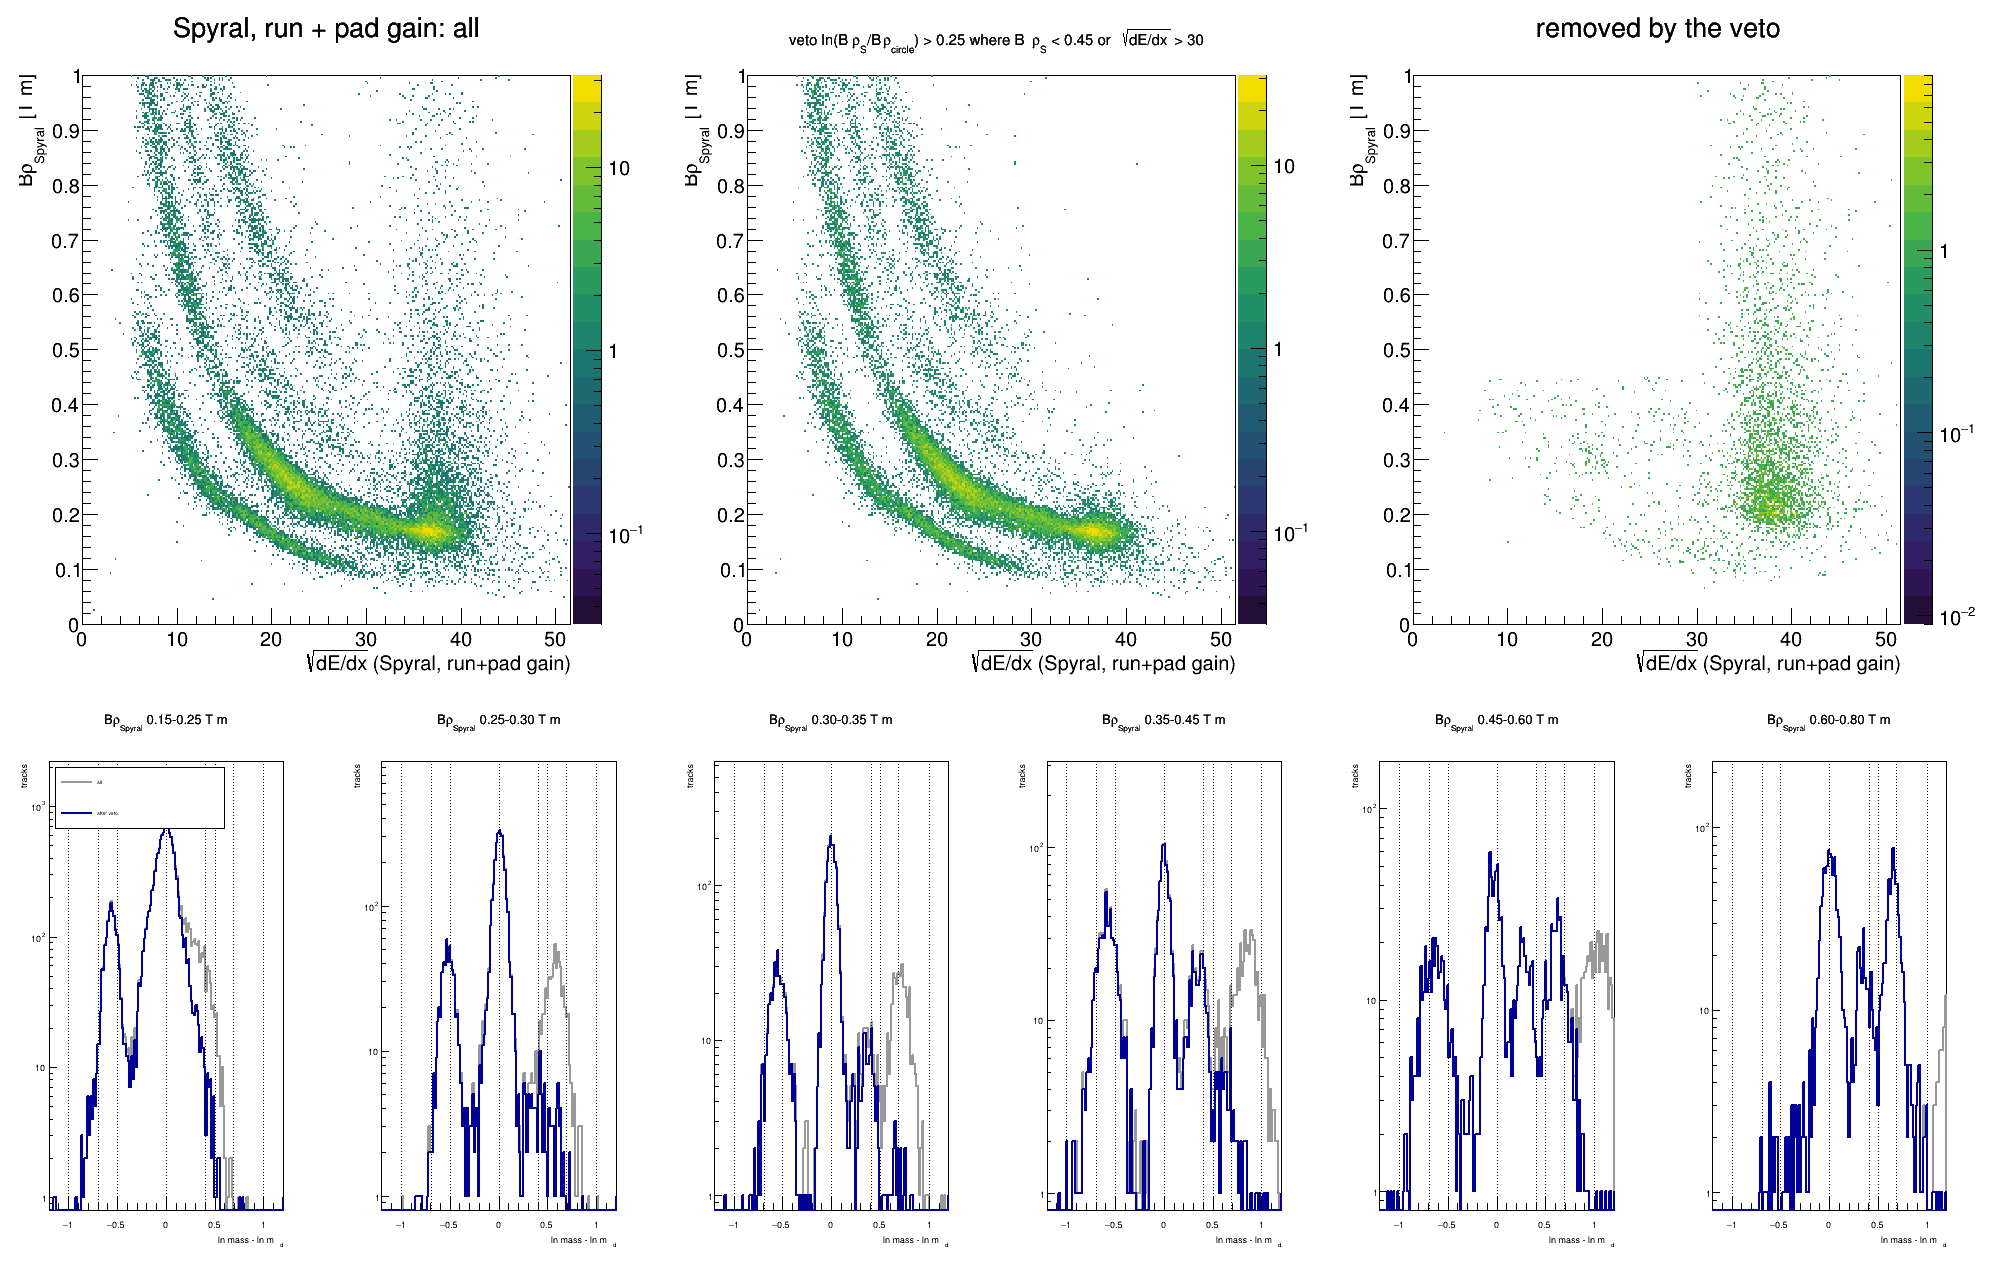
\includegraphics[width=\textwidth]{figures/pid_spyral_veto_opt2.png}
  \caption{a1975: Spyral PID before the cross-check, after it, and the rejected tracks. Bottom: ln-mass per
  \brho{} slice before (grey) and after (blue).}
  \label{fig:pid-veto}
\end{figure}

The a1975 configuration:
\begin{verbatim}
auto pid = new AtPIDTask();
pid->SetMinPoints(15);
pid->SetDedxGain(gSpyral, g3D);            // per run, from AtPIDGainTable
pid->SetPadGainMap("padgain_d2_v1.txt");
pid->GetHelix3D().SetHitRefit(true, true);
pid->GetHelix3D().SetArcAngle(true);
AtTools::AtPIDCombineOpt opt;              // lnRatioMax 0.25, maxBrho 0.45
opt.highSq = 30;                           // a1975 D2 (Spyral units)
opt.addBackScale = 0.965;                  // a1975 D2
pid->SetCombine(true, opt);
\end{verbatim}
Here \code{highSq} is in Spyral run- and pad-gain-corrected units, and \code{addBackScale} is the median ratio of the
Spyral to the 3D \sqdedx{} on tracks whose two \brho{} values agree. Both depend on the gain and must be measured for another experiment.
The implementation was validated track by track against the a1975 analysis macros on 2670 tracks
(\code{macro/Unpack\_HDF5/a1975/D2\_UKF/validate\_pid\_framework\_dp.C}).

\section{Track-quality cuts}

These depend on the species expected and stay at the analysis level, built on the stored flags.

\paragraph{Too short.} For a track that stops in the gas, the range at fixed \brho{} scales as $z^2(B\rho)^4/M^3$: a
triton's range is about 0.3 of a deuteron's at the same momentum, and no $z = 1$ or $z = 2$ ion stops shorter than a
triton. A \code{contained} track whose \code{length} is well below the lightest-range species allowed at its \brho{} is
a track-finding artefact. a1975 used $e^{-0.4}$ times the simulated triton range. The range plane is also the best
check that a \dedx{} band is real, because it does not depend on the gain (Fig.~\ref{fig:pid-range}).

\begin{figure}[htbp]
  \centering
  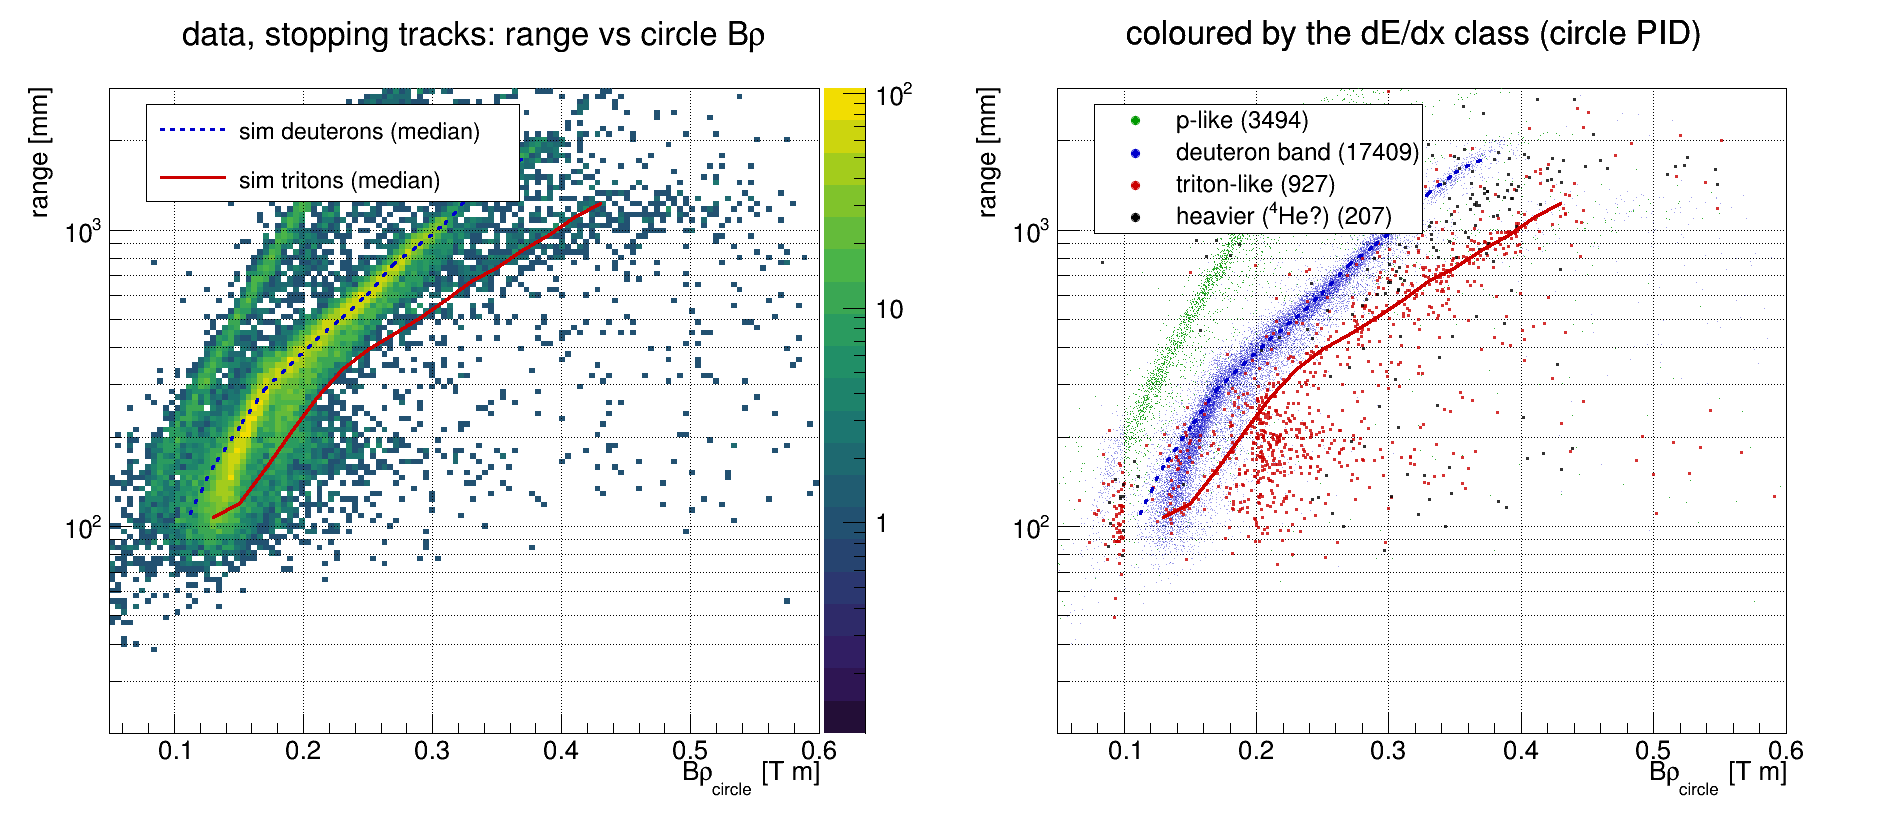
\includegraphics[width=\textwidth]{figures/pid_range_data.png}
  \caption{a1975: range against circle \brho{} for tracks that stop in the gas, with the simulated deuteron and
  triton medians; right: coloured by the \dedx{} class.}
  \label{fig:pid-range}
\end{figure}

\paragraph{Mid-track charge peak.} A candidate whose charge peaks well before its end (\code{midPeak}) is a stopped
particle with other hits attached. On a1975 this explained 67\,\% of the triton-like tracks that were shorter than
any triton. Apply the cut only in the region being purified: applied everywhere it also removes real slow deuterons
(17\,\% at 0.10--0.15~T\,m on a1975).

\section{Choosing a PID method for a new experiment}

\begin{enumerate}
\item Simulate every species that has to be separated, not only the particle of interest, and run the estimators on
  all of them. Judge separation and misidentification per \brho{} slice against truth. On a1975 a comparison against
  a computed locus led to a wrong conclusion, because the estimator biased both species alike (Fig.~\ref{fig:pid-dt}).
\item Calibrate the gain per run and per pad on the data before comparing estimators.
\item Inspect the PID plane of each estimator and the tracks one removes or moves, with event displays. Switch on the
  combination if Spyral disagrees with the 3D circle for a population.
\item Use the range plane for stopping tracks.
\item Expect the \dedx{} resolution to be the limit. On a1975, GENFIT \brho{} under either hypothesis, a truncated
  mean, averaging Spyral and 3D \dedx, and the outer pads gave no PID gain. GENFIT gives the vertex momentum once the
  species is known (Chapter~\ref{ch:fitting}).
\end{enumerate}

\begin{figure}[htbp]
  \centering
  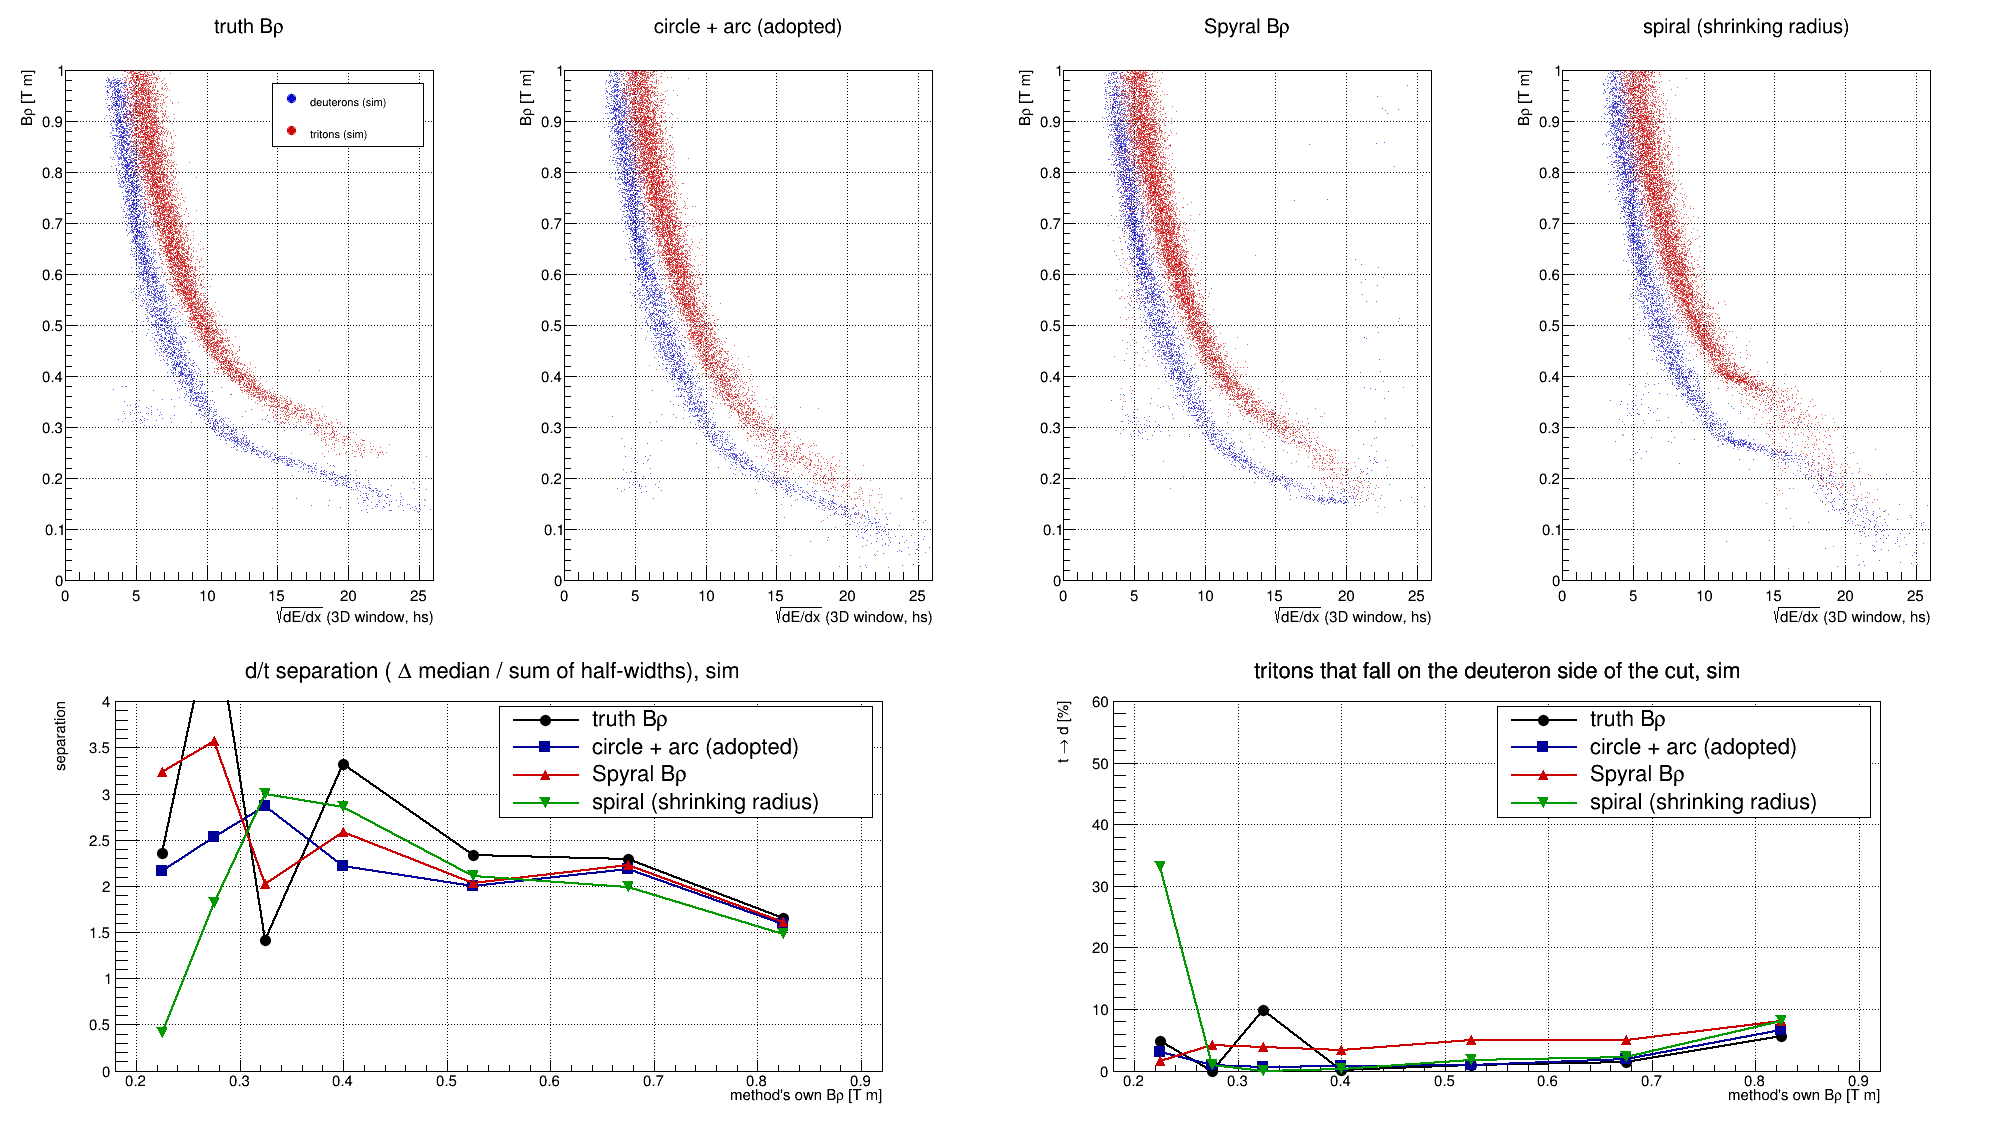
\includegraphics[width=\textwidth]{figures/pid_dt_sim.png}
  \caption{a1975: simulated deuterons (blue) and tritons (red) for each \brho{} estimator, with the separation and
  the misidentification per slice of each estimator's own \brho.}
  \label{fig:pid-dt}
\end{figure}

\section{The a1975 result}

The adopted a1975 PID is Spyral with the per-run and pad gains, the cross-check of Sec.~\ref{sec:pid-combine} with
the rejected tracks re-added, and the two quality cuts (the charge-peak cut only in the triton region). The cuts
remove 2.4\,\% of the tracks and keep 99--100\,\% of the deuteron peak (Fig.~\ref{fig:pid-final}). Protons and
deuterons are separated at all \brho; tritons are separated from deuterons above 0.35~T\,m, and at 0.25--0.35~T\,m
a triton peak sits on the deuteron tail. The full study is documented in
\code{docs/PID\_manual/pid\_a1975.pdf}.

\begin{figure}[htbp]
  \centering
  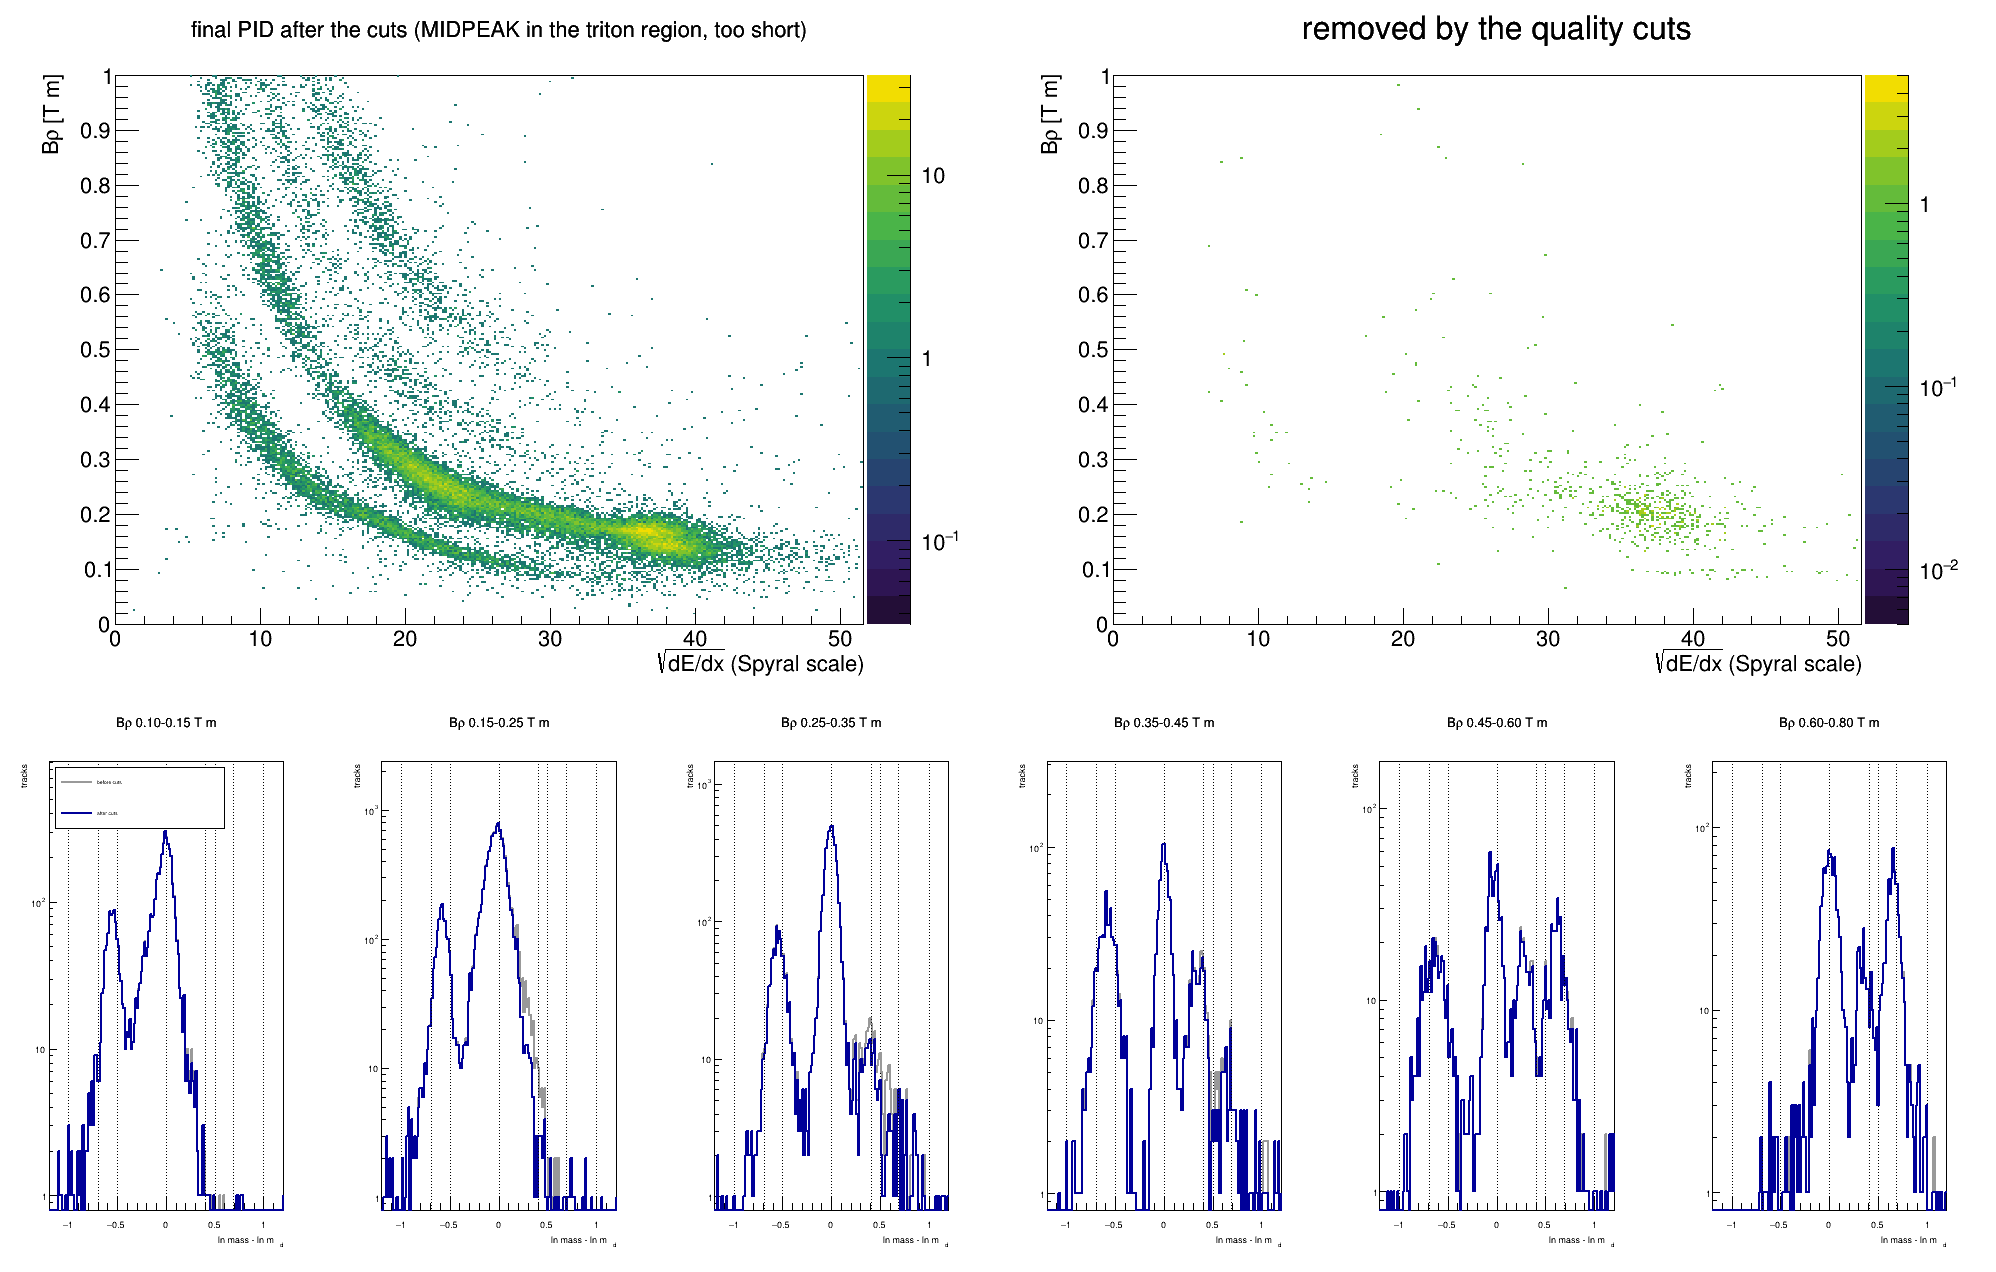
\includegraphics[width=\textwidth]{figures/pid_final_cuts_tonly.png}
  \caption{a1975 adopted PID: plane after the quality cuts and the removed tracks; bottom: ln-mass per \brho{} slice
  before (grey) and after (blue) the cuts.}
  \label{fig:pid-final}
\end{figure}

\section{Pitfalls}

\begin{itemize}
\item Gates drawn on one plane (estimator, gain correction, \code{SetMinPoints}) are not valid on another; redraw
  them whenever the PID configuration changes.
\item A \code{TTree::Draw} formula carrying per-slice lookups can exceed the operator limit of \code{TTreeFormula}
  (``Too many operators'') and silently return nothing; compute such flags in C++.
\item The PID estimators use the hit order produced by pattern recognition only through their own orderings
  (Spyral sorts by $z$, AtHelix3D builds a backbone); see Chapter~\ref{ch:patternrecognition} for the hit order.
\item \code{AtPIDEvent} version 3 adds \code{fCombined}; older files read back with it empty.
\end{itemize}
